\documentclass{ctexart}
\usepackage{amsmath}
\usepackage{amssymb}
\usepackage{graphicx}
\usepackage{gbt7714}
\usepackage{wrapfig}
\ctexset{
    % 修改 section。
    section={   
        name={,、},
        number={\chinese{section}}
    }
}

\title{在气垫导轨上研究简谐振动}
\author{陆知辰-10225301456}
\date{\today}
\graphicspath{{figure/}}

\begin{document}

\begin{titlepage}
  \centering
  % 插入图片
  
\includegraphics[width=0.5\textwidth]{ecnu.png}
  
  % 空行用于调整标题位置
  \vspace*{\baselineskip}
  
  % 标题
  \Huge\textbf{物\quad 理\quad 实\quad 验 \quad (二)}
  % 空行用于调整标题和其他信息之间的间距
  \vspace*{0.3\baselineskip}
  
  % 具体实验名称
  \huge 在气垫导轨上研究简谐振动
  
  % 空行用于调整时间和其他信息之间的间距
  \vspace*{2\baselineskip}
  
  % 时间
  \large 时间:\today
  
  % 空行用于调整时间和其他信息之间的间距
  \vspace*{\baselineskip}
  
  % 创作人
  \large 创作人:陆知辰
  
  % 空行用于调整创作人和学号之间的间距
  \vspace*{\baselineskip}
  
  % 学号
  \large 学号:10225301478
  
\end{titlepage}
\newpage
\tableofcontents
\newpage
\section{实验摘要}
  \subsection{实验概要}
  简谐振动是周期运动中最简单的运动方式。研究简谐振动是了解周期运动最简单最理想的模型。对于简谐振动而言,其动力学特征是受力情况满足$F=-kx$。其中$x$为偏离平衡位置的位移大小。
  本实验就是在气垫导轨上研究简谐子在简谐振动的时候的主要特征及其运动形式。
  \subsection{实验目的}
  1.\quad 了解简谐振动运动规律的验证方法及要求。

  2.\quad 了解简谐振动过程中的机械能守恒定律的验证方式。
  
  3.\quad 掌握对数据对结果图形的处理方式。

\section{实验原理}
  \begin{figure}[b]
    \centering
    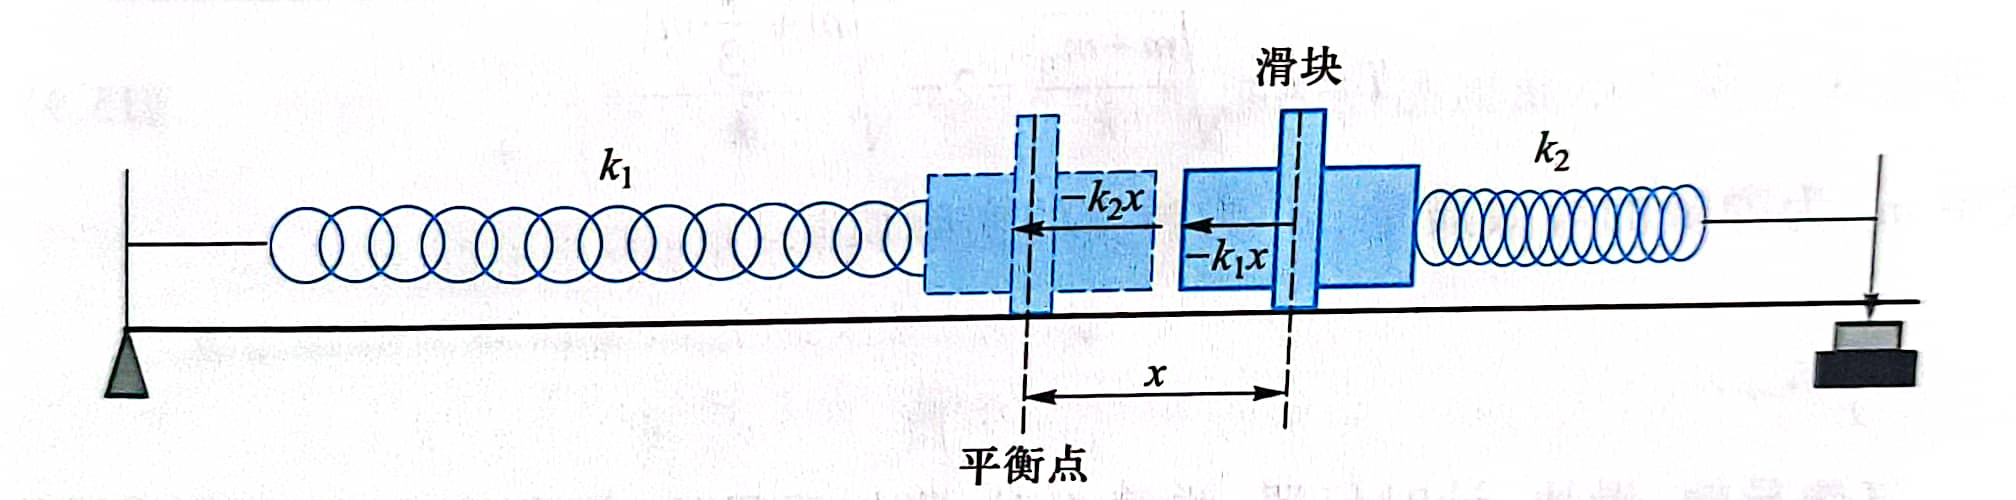
\includegraphics[height=0.3\textwidth,width=1\textwidth]{yuanli1.jpg}
    \caption{实验原理辅助用图}\label{figureyuanli1}
  \end{figure}
在如图\ref{figureyuanli1}中所展示的那样,实验器材的原理可以抽象为如图的模型。装置为一个水平的气垫导轨,不同
弹性系数的弹簧$k_{1}$和$k_{2}$各自的一端固定在两端的支架上,另一端固定在两弹簧中间的质量块上。在滑块静止后拉
动滑块使得滑块偏离平衡位置使弹簧产生弹性形变对滑块有拉力作用。对滑块进行受力分析可得当滑块偏离平衡位置的位移
为$x$的时候,所受到的回复力为
\begin{equation}
  F==(k_{1}+k_{2})x
\end{equation}
具体可以将两个弹簧视为一个整体,整体弹簧的弹性系数等于两个分弹簧的弹性系数的和即$k_{和}=k_{1}+k_{2}$。
根据上文对简谐运动特征的分析可以得出该滑块的运动是简谐运动。
这样的近似忽略了空气阻力以及其他形式的能量的损耗。以此为假设就能得出滑块就可以看作一个简谐振动子。

再根据牛顿第二定律$\ddot{a}*m=F$可以列出该滑块的动力学微分方程
\begin{equation}\label{niuerweifengfangchen}
  m\frac{d^2 y}{d x^2}=-kx 
\end{equation}
将方程解出可以得到解为
\begin{equation}\label{weiyifangchenjie}
  x=A\sin \left( \omega t+ {\varphi}_{0} \right)
\end{equation}
对于方程\ref{weiyifangchenjie}而言,式子中的$A$为振幅,${\varphi}_{0}$为初相位,
这两个量只和初始状态有关,是常数。$\omega$为振动频率,和初始状态无关,和系统本身的特征有关。
具体而言,$\omega = \sqrt{\frac{k}{m}} $,所以$\omega$只和$m$与$k$有关。并且两者都是常数。
由此通过$T=\frac{2\pi}{\omega}$可以得出振子的周期还可以表示为
\begin{equation}\label{zhouqiwutanhuang}
  T=2\pi \sqrt{\frac{m}{k}}
\end{equation}
但是上述过程中没有讨论弹簧自身的质量的影响,重新考虑弹簧自身的质量后\ref{zhouqiwutanhuang}式将改写为
\begin{equation}\label{zhouqitanhuang}
  T=2\pi \sqrt{\frac{m+m_{0}}{k}}=2\pi \sqrt{\frac{m+\frac{1}{3}m_{s}}{k}}
\end{equation}
其中\ref{zhouqitanhuang}式中的$m_{0}$为弹簧的等效质量,$m_{s}$为弹簧的实际质量。

已知以上条件后就可以推导出下列的式子

根据\ref{weiyifangchenjie}式可以得出速度的表达式为
\begin{equation}
  v=\frac{dx}{dt} =\omega A \cos \left( \omega t + {\varphi}_{0} \right)
\end{equation}

滑块的动能和振动势能为
\begin{equation}
  E_{k}=\frac{1}{2} mv^{2}=\frac{1}{2}kA^{2} {\cos}^{2}\left( \omega t + {\varphi}_{0} \right)
\end{equation}
\begin{equation}
  E_{P}=\frac{1}{2}kx^{2}=\frac{1}{2}kA^{2} {\sin}^{2} \left( \omega t + {\varphi}_{0} \right)
\end{equation}

最终可以得到总能量为
\begin{equation}
  E=E_{k}+E_{P}=\frac{1}{2}kA^{2}
\end{equation}






\section{实验装置器材介绍}
  \subsection{实验仪器}
  气垫导轨,滑块,计时仪器,弹簧数对,重物质量块,物理天平,米尺,
  若干不同当光片。
  \subsection{}

\end{document}